\mycolumnbreak
\sectionstage[2]{Zeichnen (Paket \Paket{tikz})}
Quelle:	\url{http://www.tn-home.de/TUGDD/Stuff/TikZ_final.pdf}

Hinweis vorweg: Man sollte sich gut überlegen, ob man wirklich innerhalb von LaTeX zeichnen möchte, oder ob ein Zeichenprogramm wie z.B. Inkscape besser geeignet ist.


\subsection{Basics}
\begin{lstlisting}
\usepackage{tikz} % läd intern auch das Paket pgf
\usetikzlibrary{arrows,automata,backgrounds,calendar} % bei Bedarf
??? \tikzoptions ???????	

\draw(0,0) -- (2,2); 			 %Linie
\draw[->](0,0) -- (2,2);	%Pfeil
\draw[step=0.1,gray,very thin] (0,0) grid (1,1);		% Gitter zeichnen
\draw[OPT,OPT]  ....
\end{lstlisting}

\subsubsection{OPTionen}
\begin{lstlisting}
%Pfeilsorten:
->
<-
|-> 
<-> 
>->>

%Linienstärken:
ultra thin
very thin
thin
semithick
thick
very thick
ultra thick
(help lines)
line width=12
line width=0.2cm

%Linien-Eigenschaften:
dashed
dottet
rounded corners 	%(runde Ecken)
red			(Farben: red, green, blue, cyan, magenta, yellow, black, gray, darkgray, ligthgray, brown, olive, orange, pink, purple, teal, violet, white.)	\\

%Farben:
\node[...,fill=black!60!green,...]
\node[...,fill={rgb:red,4;green,2;yellow,1},...]
% in LaTeX selbst definierte Farben können auch verwendet werden.
\end{lstlisting}

\subsubsection{Koordinaten}
\begin{lstlisting}
\draw[->] (0,0) -- (2, 2);			% absoulte Koordinaten
\draw[->] (2,0) -- +(2, 2);			% relative Koordinaten mit "+", unveränderter Referenzpunkt
\draw[->] (2,0) -- ++(2, 2);			% relative Koordinaten mit "++", veränderter Referenzpunkt
\draw (0:1cm) -- (72:1cm) -- (2*72:1cm)	% Polarkoordinaten mit (winkel:radius)
\end{lstlisting}

% ----- ----- -----------------------------
\subsection{Objekte zeichnen}
\lstinline|\begin{tikzpicture}	...	\end{tikzpicture}|

\subsubsection{Kurven zeichnen}
(\url{http://www.math.tugraz.at/~huss/new/teaching/computermathematik09/dateien/tikz_demonstration.pdf})
\begin{lstlisting}
\draw (0,0) .. controls (0,1) and (1,1) .. (2, 2);	% Direkte Eingabe der Kontrollpunkte
\draw[bend left=30] (3,0) to (4, 2);		% Die Line krümmt sich um 30 Grad nach Links
\draw[out=90, in=-90] (6,0) to (7, 2);		% aus- und eingehenden Winkel festlegen
\end{lstlisting}

\subsubsection{Ellipsen und Kreise}
\begin{lstlisting}
\draw (0,0) circle (10pt);		% Kreis
\draw (2,0) ellipse (10pt and 5pt);
\end{lstlisting}

\subsubsection{Objekte füllen}
\begin{lstlisting}
\fill (0,0) circle (0.25);
\fill[red] (1,0) circle (0.25);
\fill[blue] (2,0) circle (0.25);
\shade[ball color=green] (3,0) circle (0.25);
\fill[orange] (4,0) circle (0.25);
\fill[green,opacity=0.5] (4.25,0) circle (0.25);
\end{lstlisting}





%-------------------------------------
\columnbreak


\subsection*{Beispiel}

\begin{minipage}{0.34\linewidth}
	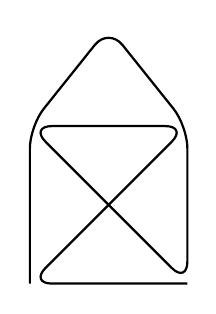
\begin{tikzpicture}[scale=0.4]
		\tikz 
		\draw[thick,rounded corners=8pt] (0,0) -- (0,2) -- (1,3.25) -- (2,2) -- (2,0) -- (0,2) -- (2,2) -- (0,0) -- (2,0);
	\end{tikzpicture}
\end{minipage}
%
%
\begin{minipage}{0.69\linewidth}
\begin{lstlisting}
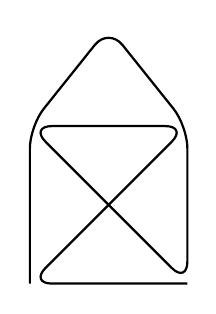
\begin{tikzpicture}[scale=0.4]
	\tikz \draw[thick,rounded corners=8pt] (0,0) -- (0,2) -- (1,3.25) -- (2,2) -- (2,0) -- (0,2) -- (2,2) -- (0,0) -- (2,0);
\end{tikzpicture}
\end{lstlisting}
\end{minipage}

\usetikzlibrary{circuits.ee.IEC}
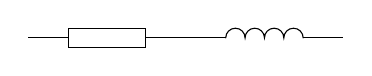
\begin{tikzpicture}[circuit ee IEC]
	\draw (0,0) to [resistor] (2,0) to [inductor] (4,0);
\end{tikzpicture}

\bigskip

%\begin{tikzpicture}[
	%circuit ee IEC,
	%x=3cm,y=2cm,
	%semithick,	
	%every info/.style={font=\footnotesize},	
	%small circuit symbols,	
	%set resistor graphic=var resistor IEC graphic,	
	%set diode graphic=var diode IEC graphic,	
	%set make contact graphic= var make contact IEC graphic]
	%
	%% Let us start with some contacts:
	%\foreach \contact/\y in {1/1,2/2,3/3.5}
	%{
		%\node [contact] (left contact \contact) at (0,\y) {};
		%\node [contact] (right contact \contact) at (1,\y) {};
	%}
	%
	%%\foreach \contact/\y in {1/1,2/2,3/3.5,4/4.5,5/5.5}
	%%{
		%%\node [contact] (left contact \contact) at (0,\y) {};
		%%\node [contact] (right contact \contact) at (1,\y) {};
	%%}
	%%\draw (right contact 1) -- (right contact 2) -- (right contact 3)
	   %%-- (right contact 4) -- (right contact 5);
	%%\draw (left contact 1) to [diode] ++(down:1)
		%%to [voltage source={near start,
												%%direction info={volt=3}},
				%%resistor={near end,ohm=3}] ++(right:1)
		%%to (right contact 1);
	%%\draw (left contact 1) to [resistor={ohm=4}] (right contact 1);
	%%\draw (left contact 1) to [resistor={ohm=3}] (left contact 2);
	%%\draw (left contact 2) to [voltage source={near start,
																%%direction info={<-,volt=8}},
											%%resistor={ohm=2,near end}] (right contact 2);
	%%\draw (left contact 2) to [resistor={near start,ohm=1},
														%%make contact={near end,info'={[red]$S_1$}}]
											%%(left contact 3);
	%%\draw (left contact 3) to [current direction'={near start,info=$\iota$},
		%%resistor={near end,info={$R=4\Omega$}}]
		%%(right contact 3);
	%%\draw (left contact 4) to [voltage source={near start, direction info={<-,volt=8}}, 		resistor={ohm=2,near end}] (right contact 4);
	%%\draw (left contact 3) to [resistor={ohm=1}] (left contact 4);
	%%\draw (left contact 4) to [resistor={ohm=3}] (left contact 5);
	%%\draw (left contact 5) to [resistor={ohm=4}] (right contact 5);
	%%\draw (left contact 5) to [diode] ++(up:1)
		%%to [voltage source={near start,
		%%direction info={volt=3}},
		%%resistor={near end,ohm=3}] ++(right:1)
		%%to (right contact 5);
%\end{tikzpicture}

%%%%%%%%%%%%%%%%%%%%%%%%%%

\sectionstage[0]{Plotten}
\lstinline|\usepackage{pgfplots}|\\
siehe \url{http://www.golatex.de/wiki/Diagramme_mit_LaTeX}\\

\noindent
\lstinline|\usepackage{filecontents}|

scale, xscale, yscale

%\begin{tikzpicture}
	%\addplot gnuplot 
  %[id=exp,mark=none,domain=0:8, very thick]{x**2+10}; 
 %\addplot gnuplot
   %[raw gnuplot,id=bal,mark=none,very thick]{
    %set xrange  [0:10];
    %f(x)=a*x+b;
    %fit f(x) "data.dat" via a,b;
    %plot f(x)};
 %\addplot plot
  %[only marks,mark=x,thick] 
  %file {data.dat};
%\end{axis} 
%\end{tikzpicture} 

\hrule \vspace{0.5\baselineskip}
%----- EOF -----